
\chapter{Cryptographic Preliminaries}
\label{chap:crypto_prelims}

Elliptic-curve cryptography (ECC) is essentially a public-key cryptography system, design of which is based on the algebraic structure of elliptic curves over finite fields \cite{Koblitz2011}.
ECC enables significant reduction in memory usage as the public-key length in ECC framework is much smaller than other public-key cryptography schemes like RSA for the same security level.
It is widely used for many applications like encryption, digital signatures, pseudo-random generators and other tasks. 

All cryptocurrencies are built on the Elliptic-curve cryptography framework.
The security of such systems depend on the security guarantees provided by the ECC framework.
We will see a couple of cryptographic assumptions which promise us the security guarantees for cryptocurrency systems.
Thus, before delving into the details of proof of reserves protocols, it is worthwhile spending some time learning about the background math of cryptocurrencies.
Note that we assume familiarity of the reader with basic concepts of group theory and modular arithmetic.
A short but sufficient primer on both of these topics in present in \cite{Sarva2017}. 


\section{Notation}
\label{scn:notation}
Let $\mathcal{G} = \{ \G, q, g \}$ be the description of a cyclic group $\G$ of prime order $q$ with generator $g$ of $\G$. Let $h\in \G$ be another random generator of $\G$ such that the discrete logarithm relation between $g$ and $h$ is not known. Let
$\G^n$ and $\Z^n_q$ be the $n$-ary Cartesian powers of sets $\G$ and $\Z_q$ respectively.
%TODO: Check the second part of the following statement.
% Yes, it is.
Group elements which are Pedersen commitments are denoted by uppercase letters and randomly chosen group elements are denoted by lowercase letters.
% TODO: Check if the following statement is true after the rewrite.
% It is true and necessary too. Matrix description not necessary, so removing it.
Bold font denotes vectors.
Inner product of two vectors $\textbf{a}, \textbf{b} \in \Z_q^n$ is defined as $\langle \textbf{a},\textbf{b} \rangle \coloneqq \sum_{i=1}^{n} a_i \cdot b_i$ where $\textbf{a}=(a_1,\dots, a_n), \textbf{b}=(b_1,\dots,b_n)$. Further, Hadamard and Kronecker products are defined respectively as, $\textbf{a} \circ \textbf{b} \coloneqq (a_1 \cdot b_1, \dots, a_n \cdot b_n) \in \mathbb{Z}_q^n$, $\textbf{a} \otimes \textbf{c} \coloneqq (a_1 \textbf{c}, \dots, a_n \textbf{c}) \in \mathbb{Z}_q^{nm}$ where $\textbf{c} \in \mathbb{Z}_q^m$. For a base vector $\textbf{g} = (g_1, \dots, g_n) \in \G^n$, vector exponentiation is defined as $\textbf{g}^{\textbf{a}} = \prod_{i=1}^{n}g_i^{a_i} \in \G$. For a scalar $u \in \Z_q^{\ast}$, we denote its consecutive powers in the form of a vector $\vecnb{u}^{n} \coloneqq (1, u, u^2, \dots, u^{n-1})$.
To represent the exponentiation of all components of a vector $\textbf{a}$ by the same scalar $k \in \Z_q$, we use $\textbf{a}^{\circ k}$ to mean $(a_1^k, a_2^k, \ldots,a_n^{k})$.
If an element $a$ is chosen uniformly from a set $A$, such a choice is denoted by $a \rgen A$.
We denote the relation \emph{Relation} using the specified input and witness as $\{ (Public \ Input; \ Witness): Relation \}$.
We refer to $\mathcal{A}$ as a \textsf{PPT} adversary which is a probabilistic Turing Machine that runs in polynomial time in the security parameter $\lambda$.
An \emph{interactive proof} for the decision problem $\pi$ is described as follows:
\begin{enumerate}
    \item There are two participants, a prover $\P$ and a verifier $\V$.
    \item The proof consists of a specified number of rounds.
    \item In the beginning, both participants get the same input.
    \item In each round, the verifier challenges the prover, and the prover responds
    to the challenge.
    \item Both the verifier and the prover can perform some private computation.
    \item At the end, the verifier states whether he was convinced or not.
\end{enumerate}


\section{Basics of Elliptic Curves}
\label{scn:ECC}

Let $a, b \in \Rn$ such that $4a^3 + 27b^2 \neq 0$. Let $E$ be the set of solutions $(x,y) \in \Rn$ to the equation
\begin{equation}
    y^2 = x^3 + ax + b.
\end{equation}
An elliptic curve over $\Rn$ is given by the set $E \cup \{\Inf\}$ where $\Inf$ is known as the \textit{point at infinity}.
An example of an elliptic curve over $\Rn$ is given in Figure \ref{fig:ecc}.
Note that the condition $4a^3 + 27b^2 \neq 0$ ensures that the curve does not have repeating roots.
This condition is necessary in the discussion of elliptic curve groups.


\begin{figure}
    \begin{center}
        \tikzsetnextfilename{eg_ecc}
        \begin{tikzpicture}
            \begin{axis}[
                axis lines = center,
                xlabel = $x$,
                ylabel = {$y$},
                ymin=-5, ymax=5,
                xmin=-4,xmax=4,
            ]
            %First EC - positive y
            \addplot [
                domain=-3:3, 
                samples=10000, 
                color=red,
            ]
            {sqrt(x^3 - x + 2)};
            %First EC - negative y
            \addplot [
                domain=-3:3, 
                samples=10000, 
                color=red,
            ]
            {-sqrt(x^3 - x + 2)};
            \end{axis}
        \end{tikzpicture}
        \caption{An elliptic curve given by the equation $y^2 = x^3 - x + 2$ over $\Rn$}
        \label{fig:ecc}
    \end{center}
\end{figure}

\subsection{Point Addition in Elliptic Curves}

The set $E \cup \{\Inf\}$ needs to be an algebraic group for us to be able to define operations on it.
Thus, we define a group operation over $E \cup \{\Inf\}$ known as \textit{point addition}.
Suppose we have two points $P = (x_1, y_1), Q = (x_2,y_2) \in \Rn \times \Rn$ such that $x_1 \neq x_2$. 
We show them by blue and yellow coloured points in Figure \ref{fig:point_add}(a).
We draw a line passing through $P$ and $Q$. 
As the degree of an elliptic curve equation is 3, any non-tangent line must intersect the curve in 3 distinct points.
Suppose the line passing through $P$ and $Q$ intersects the curve at point $R^{\prime} = (x_3, -y_3) \in \Rn \times \Rn$, shown in orange colour.
We define the result of point addition of points $P$ and $Q$ to be the point $R$ which is the mirror reflection of $R^{\prime}$.
Therefore, we have $R = (x_3, y_3)$ shown in red colour. 
Simple calculation shows that given $P = (x_1,y_1), Q = (x_2, y_2)$ and $x_1 \neq x_2$, point addition gives us $P+Q = (x_3, y_3)$ such that
\begin{equation}
    x_3 = \left( \frac{y_2-y_1}{x_2-x_1} \right)^2 -x_1 -x_2, \ y_3 = \left( \frac{y_2-y_1}{x_2-x_1} \right) (x_1 - x_3) - y_1.
    \label{eqn:point_add}
\end{equation}

\begin{figure}[h!]
    \begin{center}
        \tikzsetnextfilename{point_add1}
        \begin{tikzpicture}
            \begin{groupplot}[
                axis lines = center,
                xlabel = $x$,
                ylabel = {$y$},
                ymin=-4, ymax=4,
                xmin=-3,xmax=3,
                ticks=none,
                group style={group name=point_add, group size=2 by 1, horizontal sep=2.2cm},
                width=0.52\textwidth]
            \nextgroupplot
            %First EC - positive y
            \addplot [
                domain=-3:3, 
                samples=10000, 
                color=red,
            ]
            {sqrt(x^3 - x + 2)};
            %First EC - negative y
            \addplot [
                domain=-3:3, 
                samples=10000, 
                color=red,
            ]
            {-sqrt(x^3 - x + 2)};
            \addplot[scatter,scatter src=explicit,dashed, mark=*] coordinates { 
                (-1.39,0.894) [1] 
                (-0.27,1.5) [2] 
                (2.008,2.844) [3]
                (2.008,-2.844) [4]
            };
            \nextgroupplot
            %First EC - positive y
            \addplot [
                domain=-3:3, 
                samples=10000, 
                color=red,
            ]
            {sqrt(x^3 - x + 2)};
            %First EC - negative y
            \addplot [
                domain=-3:3, 
                samples=10000, 
                color=red,
            ]
            {-sqrt(x^3 - x + 2)};
            \addplot[scatter,scatter src=explicit,dashed, mark=*] coordinates { 
                (-1,-6) [4]   
                (-1,-1.414) [2]  
                (-1,1.414) [1] 
                (-1,6) [3]
                
            };
        \end{groupplot}
        \node[text width=4cm,align=center,anchor=north] at ([yshift=2mm]point_add c1r1.south) {\captionof*{subfigure}{(a) $x_1 \neq x_2$\label{subfig:ecc1}}};
        \node[text width=4cm,align=center,anchor=north] at ([yshift=2mm]point_add c2r1.south) {\captionof*{subfigure}{(b) $x_1 = x_2, y_1 = -y_2$\label{subfig:ecc2}}};
        \end{tikzpicture}
        
        \tikzsetnextfilename{point_add2}
        \begin{tikzpicture}
            \begin{axis}[
                axis lines = center,
                xlabel = $x$,
                ylabel = {$y$},
                ymin=-5, ymax=5,
                xmin=-4,xmax=4,
                ticks=none,
            ]
            %First EC - positive y
            \addplot [
                domain=-3:3, 
                samples=10000, 
                color=red,
            ]
            {sqrt(x^3 - x + 2)};
            %First EC - negative y
            \addplot [
                domain=-3:3, 
                samples=10000, 
                color=red,
            ]
            {-sqrt(x^3 - x + 2)};
            \addplot[scatter,scatter src=explicit,dashed, mark=*] coordinates { 
                (-0.92,1.463) [1]   
                (2.117,3.06) [3]  
                (2.117,-3.06) [4] 
            };
            \end{axis}
        \end{tikzpicture}
        \captionof*{subfigure}{(c) $x_1 = x_2, y_1 = y_2 \neq 0$}
    \end{center}
    \caption{Point addition in elliptic curves over $\Rn$}
    \label{fig:point_add}
\end{figure}

Now if $P$ and $Q$ are such that $x_1 = x_2$ but $y_1 = -y_2$, the line passing through $P$ and $Q$ is vertical and possibly intersects the curve at infinity.
In this case, we define the point addition operation as $P + Q = \Inf$.
Therefore, the special point $\Inf$ acts as an identity point in the group $E \cup \{\Inf\}$.
Further, if we have $P=Q$, i.e. $x_1 = x_2, y_1 = y_2 \neq 0$, we draw tangent to the curve at point $P$.
As the degree of the curve is 3, any tangent will intersect the curve at one and only one point, say point $R^{\prime}$.
The result $R$ in this case is again the mirror reflection of point $R^{\prime}$ about the x-axis. 
The addition of a point to itself is known as \textit{point doubling}. 
The explicit formula for point doubling of point $P=(x_1,y_1)$ can be written as $P+P = 2P = (x_2, y_2)$ such that
\begin{equation}
    x_2 = \left( \frac{3x_1^2 + a}{2y_1} \right)^2 - 2x_1, \ y_2 = \left( \frac{3x_1^2 + a}{2y_1} \right)(x_1-x_2) - y_1.
    \label{eqn:point_double}
\end{equation}

The point addition operation is closed in the set $E \cup \{\Inf\}$ by construction. 
Further, $\Inf$ acts as an identity element in the set $E \cup \{\Inf\}$.
For each point $P \in E$, we can find its \textit{inverse} $Q \in E$ as its reflection about the x-axis as for such cases, we have $P+Q = \Inf$.
Therefore, the set $E \cup \{\Inf\}$ is a group under point addition.

In practice, we use elliptic curves over finite fields instead of real numbers.
The group operations are now defined over an underlying finite field $F$. 
The division by a non-zero field element $x \in F$ is interpreted as multiplication by its multiplicative inverse $x^{-1}$.
Similarly, subtraction of a field element $x \in F$ is interpreted as addition by its additive inverse $-x$.
This is the basis of the elliptic curve cryptography used in modern day systems except that of 
For example, Bitcoin and Grin cryptocurrency systems use the prime-ordered elliptic curve \texttt{secp256k1} \cite{Hess2000}.

Note that from hereon we use multiplicative notation to denote group operation on elliptic curves $\G$ on finite fields $\F_q$ for a large prime $q$. 
Lastly, addition of a point $P \in \G$ for $k$ times is shown as scalar multiplication in additive notation and exponentiation in multiplicative respectively.
\begin{equation*}
    \underbrace{P + P + \dots + P}_{k \text{ times}} = kP \in \G.
\end{equation*}
Similarly, in multiplicative notation, such an operation is called as exponentiation and is shown below 
\begin{equation*}
    \underbrace{P \cdot P \cdot \ldots \cdot P}_{k \text{ times}} = P^k \in \G.
\end{equation*}

\section{Cryptographic Assumptions}
\label{scn:assumptions}

Every practical cryptographic system is built on certain hardness assumptions.
For example, the widely popular RSA digital signature algorithm was based on the assumption that it computationally hard to factorize big primes \cite{RSA1978}.  
Elliptic curve cryptography is similarly based on the assumption that the \textit{Discrete Log Problem} is difficult to be solved by a computationally bounded adversary.


\begin{defn}[Discrete Log Relation]
    For all PPT adversaries $\mathcal{A}$ and for all $n\ge2$, $\exists$ a negligible function $\mu (\lambda)$ s.t
    \begin{equation*}
        \Pr 
        \Big[
        \begin{tabular}{ll}
             $\G = Setup(1^{\lambda}), g_1, \dots, g_n \leftarrow \ \G$ ;
             &
             \multirow{2}{*}{$\text{:} \exists a_i \neq 0 \wedge \prod_{i=1}^{n} g_{i}^{a_i} = 1$}\\
             $a_1, \dots, a_n \in \ \Z_p \leftarrow \mathcal{A}(\G, g_1, \dots, g_n)$
             & 
        \end{tabular}
        \Big] 
      \leq \mu(\lambda)
    \end{equation*}
   
    \vspace{0.2mm}
\end{defn} 
We say $\prod_{i=1}^{n} g_{i}^{a_i} = 1$ is a non trivial discrete log relation between $g_1, \dots, g_n$. If the Discrete Log Relation assumption stands, it implies that no \textsf{PPT} adversary can find a non-trivial relation between randomly chosen group elements. 
This is known as the Discrete Log Problem.

We use additional cryptographic assumptions such as Decisional Diffie-Hellman and its variants as described in \cite{Lai2019}.

\section{Cryptographic Commitments}

Cryptographic commitments are an important preliminary widely used to anonymise data like amounts.
We also briefly discuss some key properties of commitments of our interest. 

\begin{defn}[Commitments]
    A non-interactive commitment consists of two PPT algorithms {\normalfont(Setup, Com)}. For a message $x \in {\normalfont \textbf{M}_{pp}}$ (message space), the algorithm proceeds as follows:
    \begin{enumerate}
    \setlength\itemsep{0.3em}
        \item public parameters $pp \leftarrow {\normalfont Setup}(1^{\lambda})$ for security paramter $\lambda$
        \item {\normalfont Com}$_{pp} : {\normalfont \textbf{M}_{pp}} \times {\normalfont \textbf{R}_{pp}} \rightarrow {\normalfont \textbf{C}_{pp}}$, 
        where ${\normalfont \textbf{R}_{pp}}$ is randomness space
        \item $r \leftarrow {\normalfont \textbf{R}_{pp}}$ and compute {\normalfont \textbf{com}} = {\normalfont Com}$_{pp}(x;r)$
    \end{enumerate}
\end{defn}

\begin{defn}[Homomorphic Commitments]
    A homomorphic commitment is a non-interactive commitment such that ${\normalfont \textbf{M}_{pp}}$, ${\normalfont \textbf{R}_{pp}}$, ${\normalfont \textbf{C}_{pp}}$ are all abelian groups, and $\forall \ x_1, x_2 \in {\normalfont \textbf{M}_{pp}}$, $r_1, r_2 \in {\normalfont \textbf{R}_{pp}}$, we have 
\end{defn}
\begin{equation*}
    \text{Com}(x_1; r_1) + \text{Com}(x_2; r_2) = \text{Com}(x_1+ x_2; r_1+r_2)
\end{equation*}

\begin{defn}[Hiding Commitment]
    A commitment scheme is said to be hiding if for all PPT adversaries $\mathcal{A}$, $\exists \mu(\lambda)$, a negligible function such that,  
\end{defn}
\begin{equation*}
        \Bigg|
        \Pr
        \Bigg[
        \begin{tabular}{c | l}
             \multirow{3}{*}{$\textit{b'=b}$} 
             &
             $\textit{pp} \leftarrow \text{Setup}(1^{\lambda})$;\\
             &
             $(\textit{x}_0,x_1) \in \text{\textbf{M}}_{pp}^2 \leftarrow \mathcal{A}(pp), \
             b \leftarrow \{0,1\}, \ 
             r \leftarrow \text{\textbf{R}}_{pp},$ \\
             &
             $\textbf{com} = Com(\textit{x}_b; r),\ b' \leftarrow \mathcal{A}(pp, \ \textbf{com})$
        \end{tabular}
        \Bigg]
        - \frac{1}{2}
        \Bigg|
        \leq \mu(\lambda)
\end{equation*}
\textit{where the probability is over $b', r, Setup \ \text{and} \ \mathcal{A}$. For perfectly hiding schemes, $\mu(\lambda)=0$.}

In simple words, a commitment scheme is \textit{hiding} if it is impossible for a computationally bounded adversary to find what the message is hidden in a commitment or what randomness was used in computing the commitment.

\begin{defn}[Binding Commitment]
    A commitment scheme is said to be binding if for all PPT adversaries $\mathcal{A}$, $\exists \mu(\lambda)$, a negligible function such that,
\end{defn}
\begin{equation*}
        \Pr 
        \Bigg[
        \begin{tabular}{c | c}
             \multirow{2}{*}{$\text{Com}(\textit{x}_0;r_0)= \text{Com}(\textit{x}_1;r_1) \wedge x_0 \neq x_1$} 
             &
             $\textit{pp} \leftarrow \text{Setup}(1^{\lambda})$,\\
             &
             $\textit{x}_0, x_1, r_0, r_1 \leftarrow \mathcal{A}(pp)$
        \end{tabular}
        \Bigg] 
        \leq \mu(\lambda)
\end{equation*}
\textit{where the probability is over Setup and $\mathcal{A}$. Again, if $\mu(\lambda)=0$ then we say the scheme is perfectly binding.}

A commitment scheme is known as \textit{binding} if it is impossible for a computationally bounded adversary to change the message a commitment commits to once it has published the commitment to the original message.

\begin{defn}[Pedersen Commitment]
    ${\normalfont \textbf{M}}_{pp}, {\normalfont \textbf{R}}_{pp} = \mathbb{Z}_p$, ${\normalfont \textbf{C}}_{pp} = \mathbb{G}$ of \\order $p$.
    \begin{enumerate}
        \item {\normalfont Setup}: $g, h \leftarrow \mathbb{G}$
        \item {\normalfont Com}$(x; r) = (g^x h^r)$
    \end{enumerate}
\end{defn}

\begin{defn}[Pedersen Vector Commitment]
    {\normalfont \textbf{M}}$_{pp} = \mathbb{Z}_p^n$, {\normalfont \textbf{R}}$_{pp} = \mathbb{Z}_p$, ${\normalfont \textbf{C}}_{pp} = \mathbb{G}$ of order $p$.
    \begin{enumerate}
        \item {\normalfont Setup}: \textbf{g} $= (g_1, \dots, g_n), h \leftarrow \mathbb{G}$
        \item {\normalfont Com}$(\textbf{x} = (x_1, \dots, x_n); r) = (h^r \textbf{g}^{\textbf{x}})$
    \end{enumerate}
\end{defn}

The Pedersen vector commitment is \textit{perfectly hiding} and \textit{computationally binding} under the
discrete logarithm assumption. This means that no matter how much computational power an adversary possesses, he cannot find the message hidden in a Pedersen commitment.
Further, for a computationally bounded adversary, it is infeasible to find another opening to a Pedersen commitment once he has committed it to original message.

\section{Zero-Knowledge Arguments of Knowledge}

Zero knowledge proofs are a powerful cryptographic tool which allow a prover to prove the validity of an assertion without revealing any other information about the secret owned.
We give the formal definitions of zero knowledge proofs and their properties along with an example.
In a formal context, a \textit{proof} implies security guarantees against any adversary while security of an \textit{argument} stands valid only for a computationally bounded adversary.  
From hereon, we will interchangeably use the terms \textit{proof} and \textit{argument} as we consider only \textsf{PPT} adversaries.


\subsection{Zero-Knowledge Arguments}

A protocol in which a prover convinces a verifier that a statement
is true \textit{without} revealing any information about why it holds is known as a Zero-knowledge argument. An argument is a proof only if the prover is computationally bounded and some computational hardness holds. Hereafter, we use the terms \textit{proof} and \textit{argument} interchangeably. 

We illustrate the idea of zero-knowledge arguments of proof using the example of \textit{Ali-Baba's secret cave}\footnote{Figure courtesy: \url{https://en.wikipedia.org/wiki/Zero-knowledge_proof}.} \cite{jean89}.

\begin{figure}[h!]
    \centering
    \begin{subfigure}[b]{0.8\textwidth}
    \centering
        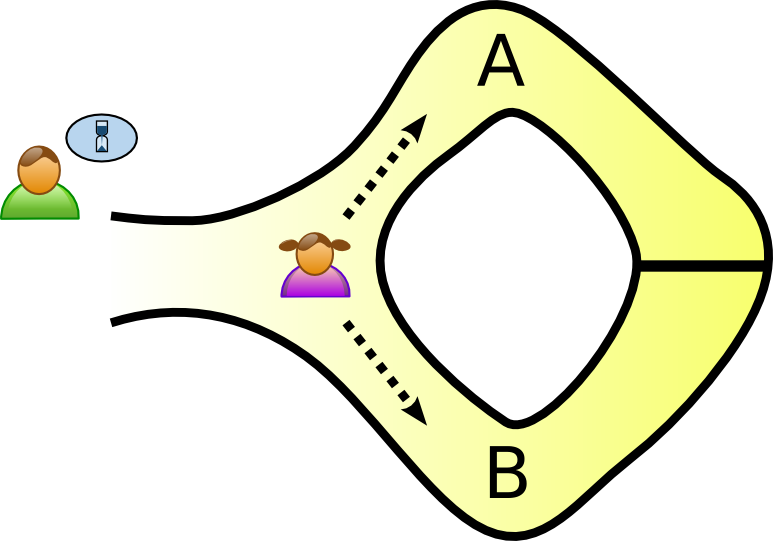
\includegraphics[width=0.44\textwidth]{Figures/Zkip_alibaba1.png}
        \label{fig:zkp1}
        \caption{Peggy chooses a path uniformly from $A, B$ without Victor knowing.}
    \end{subfigure}
    \\
    \begin{subfigure}[b]{0.8\textwidth}
    \centering
        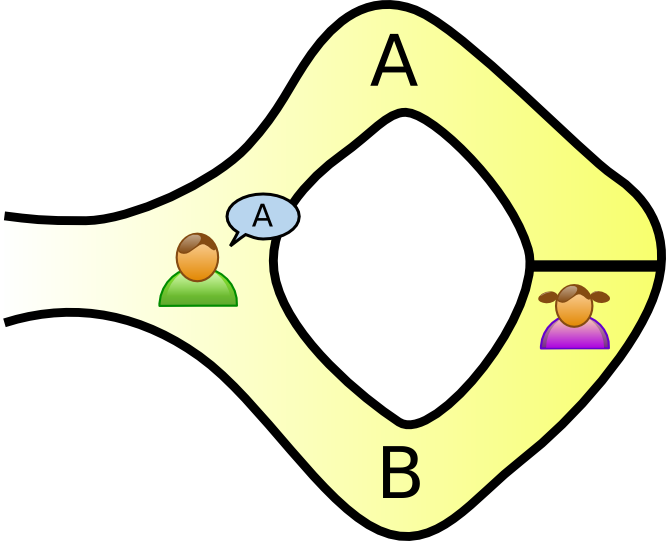
\includegraphics[width=0.4\textwidth]{Figures/Zkip_alibaba2.png}
        \label{fig:zkp2}
        \caption{Victor asks her to come out of the cave from path $A$.}
    \end{subfigure}
    \\
    \begin{subfigure}[b]{0.8\textwidth}
    \centering
        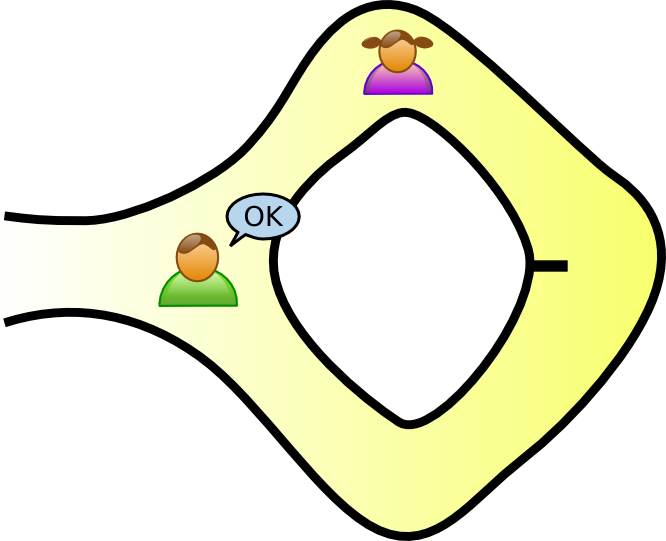
\includegraphics[width=0.4\textwidth]{Figures/Zkip_alibaba3.png}
        \label{fig:zkp3}
        \caption{If Peggy had entered from path $A$, she returns trivially. Otherwise, she could open the door using the secret key and return from path $A$.}
    \end{subfigure}
    
    \caption{Example of a zero knowledge proof}
    \label{fig:zkp_alibaba}
    \end{figure}
    
In the above example, Peggy knows the secret word used to open a mysterious door in a cave. The cave is shaped like a horse-hoe. The entrance is on one side and the magic door blocking the opposite side. Victor wants to know whether Peggy knows the secret word; but Peggy, does not want to reveal her knowledge (the secret word) to Victor or to reveal the fact of her knowledge to anyone in the world. 

Peggy and Victor run the protocol described in figure \ref{fig:zkp_alibaba}. Provided she really does know the magic word, and the path she enters and path Victor asks her to come from are same, then it's trivial for Peggy to succeed and Victor to believe that she actually knows the secret key. Further, if the chosen path by Peggy and asked by Victor doesn't match, even then she could open the door and return from a desired path. If they were to repeat this protocol many times, say 15 times in a row, her chance of successfully "guessing" all of Victor's requests would become exponentially small (about three in a lakh).

For zero-knowledge arguments presented in this report, we will consider arguments consisting of three interactive probabilistic polynomial time algorithms $(\text{Setup}, \mathcal{P}, \mathcal{V})$. These algorithms are described by:
\begin{enumerate}
    \item Setup: $\sigma \leftarrow \text{Setup}(1^{\lambda})$, $\sigma$ is common reference string
    \item $\mathcal{P}$: prover, $\mathcal{V}$: verifier
    \item Transcript $tr \leftarrow \langle \mathcal{P}, \mathcal{V} \rangle$
    \item $\langle \mathcal{P}, \mathcal{V} \rangle = b$, $b=0$ if the verifier rejects or $b=1$ accepts 
\end{enumerate}

Further, we define the relation $\mathcal{R}$ and the CRS-dependent language as:
\begin{align*}
    \mathcal{R} &:= \{ (\sigma, u, w) \in \{0,1\}^{\ast} \times  \{0,1\}^{\ast} \times  \{0,1\}^{\ast}: \ w \ \text{is a witness for}\ u \ | \ \sigma \}\\
    \mathcal{L}_{\sigma} &:=  \{ x \ | \exists w \in (\sigma, u, w) \in \mathcal{R} \}
\end{align*}

So, $\mathcal{L}_{\sigma}$ is essentially the set of statements $x$ that have a witness $w$ in the relation $\mathcal{R}$. 

\subsection{Defining Zero-Knowledge Arguments of Knowledge}
\label{subsec:zka/d_aok}
To mathematically define the notion of zero-knowledge and zero-knowledge arguments, we will provide the necessary definitions below.

\begin{defn}[Argument of Knowledge]
        The triple $(\text{Setup}, \mathcal{P}, \mathcal{V})$ is called an argument of knowledge for relation $\mathcal{R}$ if it is perfectly complete and has computational witness-extended emulation.
\end{defn}

\begin{defn}[Perfect completeness]
    $(\text{Setup}, \mathcal{P}, \mathcal{V})$ has perfect completeness if for all non-uniform polynomial time adversaries $\mathcal{A}$

    \begin{equation*}
    \Pr 
    \Big[
    \begin{tabular}{c | l}
         \multirow{2}{*}{$(\sigma, u, w) \not \in \mathcal{R} \ or \ 
         \langle \mathcal{P}(\sigma, u, w), \mathcal{V}(\sigma, u) \rangle = 1$}
         & $\sigma \leftarrow \text{Setup}(1^{\lambda})$
         \\
         & 
         $(u, w) \leftarrow \mathcal{A}(\sigma)$
    \end{tabular}
    \Big] 
    = 1
\end{equation*}
\end{defn}

\emph{Perfect completeness} implies that if a statement is actually true, then an honest verifier is convinced with probability $1$ about the truth of the statement by an honest prover.

\begin{defn}[Computational Witness-Extended Emulation]
    $(\text{Setup}, \mathcal{P}, \mathcal{V})$ has witness-extended
    emulation if for all deterministic polynomial time $P^{*}$ there exists an expected polynomial time
    emulator $\mathcal{E}$ such that for all pairs of interactive adversaries $\mathcal{A}_1 , \mathcal{A}_2$ there exists a negligible function
    $\mu (\lambda)$ such that
    
    \begin{multline*}
    \Bigg|
        \Pr
        \Bigg[
        \begin{tabular}{c | l}
             \multirow{3}{*}{$\mathcal{A}_1(tr) = 1$}
             & $\sigma \leftarrow \text{Setup}(1^{\lambda},)$
             \\
             & 
             $(u, s) \leftarrow \mathcal{A}_2(\sigma),$
             \\
             & $tr \leftarrow \langle (\mathcal{P}^{*}(\sigma, u, s), V(u, s) \rangle$
        \end{tabular}
        \Bigg]
        -\\
        \Pr 
        \Bigg[
            \begin{tabular}{l | l}
                \multirow{2}{*}{$\mathcal{A}_1(tr) = 1 \wedge$}
                &
                $\sigma \leftarrow \text{Setup}(1^{\lambda},)$
                \\
                & 
                $(u, s) \leftarrow \mathcal{A}_2(\sigma),$
                \\
                $(tr\ accepted \implies (\sigma, u, w)\in \mathcal{R})$
                &
                $(tr, w) \leftarrow \mathcal{E}^{\mathcal{O}}(\sigma, u)$
           \end{tabular}
           \Bigg]
    \Bigg|
    \leq \mu(\lambda)
    \end{multline*}
    
    where the oracle is given by  $\mathcal{O} = \langle (\mathcal{P}^{*}(\sigma, u, s), V(u, s) \rangle$, and permits rewinding to a specific point and
    resuming with fresh randomness for the verifier from this point onwards. We can also define com-
    putational witness-extended emulation by restricting to non-uniform polynomial time adversaries
    $\mathcal{A}_1$ and $\mathcal{A}_2$.       
    
\end{defn}

\textit{Computational witness-extended emulation} implies that when an adversary produces an argument to convince the verifier with some probability, then we have a corresponding emulator producing identically distributed argument with same probability, but also a witness.

\begin{defn}[Public coin]
    An argument of knowledge  $(\text{Setup}, \mathcal{P}, \mathcal{V})$ is called public coin if all messages sent from the verifier to the prover are chosen uniformly at random and independent of the prover's messages, i.e., the challenges correspond to the verifier's randomness $\rho$.
\end{defn}

\begin{defn}[Zero Knowledge Argument of Knowledge]
    An argument of knowledge $(\text{Setup}, \mathcal{P}, \mathcal{V})$ is zero knowledge if it reveals no information about $w$ apart from what could be deduced from the fact that $(\sigma, u, w) \in \mathcal{R}$.
\end{defn}

An argument of knowledge is zero knowledge if it does not leak information about $w$ apart from what can be deduced from the fact that $(\sigma, u, w) \in \mathcal{R}$. More explicitly, we note that, a zero knowledge argument of knowledge ensures that no \textsf{PPT} adversary (or verifier) can ever recover $w$ given it's relation with $\sigma, u$.

\begin{defn}[Perfect Special Honest-Verifier Zero-Knowledge]
    A public coin argument of knowledge $(\text{Setup}, \mathcal{P}, \mathcal{V})$ is a perfect special honest verifier zero knowledge (SHVZK) argument of knowledge for $\mathcal{R}$ if there exists a probabilistic polynomial time simulator $\mathcal{S}$ such that for all pairs of interactive adversaries $\mathcal{A}_1 , \mathcal{A}_2$
    
    \begin{multline*}
    \Pr
    \Bigg[
    \begin{tabular}{c | l}
        \multirow{3}{*}{$(\sigma, u, w) \in \mathcal{R} \wedge \mathcal{A}_1(tr) = 1$}
         & $\sigma \leftarrow \text{Setup}(1^{\lambda},)$
         \\
         & 
         $(u, w, \rho) \leftarrow \mathcal{A}_2(\sigma),$
         \\
         & $tr \leftarrow \langle (\mathcal{P}(\sigma, u, s), V(\sigma, u; \rho) \rangle$
    \end{tabular}
    \Bigg]
    \\
    =\Pr
    \Bigg[
    \begin{tabular}{c | l}
        \multirow{3}{*}{$(\sigma, u, w) \in \mathcal{R} \wedge \mathcal{A}_1(tr) = 1$}
         & $\sigma \leftarrow \text{Setup}(1^{\lambda},)$
         \\
         & 
         $(u, w, \rho) \leftarrow \mathcal{A}_2(\sigma),$
         \\
         & $tr \leftarrow \mathcal{S}(u, \rho)$
    \end{tabular}
    \Bigg]
    \end{multline*}

\end{defn}

PSHVZK AoK implies that even if an adversary chooses a
distribution over statements and witnesses, it isn't able to
distinguish between simulated transcript and honestly generated
transcript for $u \in \mathcal{L}_{\sigma}$.

We will be using these definitions of Zero knowledge argument and its properties in the discussion further without redefining them, unless explicitly stated.




